\documentclass{article}

\usepackage{graphicx}
\usepackage{tikz}
\usepackage{tikzsymbols}
\usetikzlibrary{calc,patterns,shapes.geometric}
\pagestyle{empty}
\usepackage[margin=0pt]{geometry}
\geometry{papersize={14in,12in}}

\def\centerarc[#1](#2)(#3:#4:#5){\draw[#1] ($(#2)+({#5*cos(#3)},{#5*sin(#3)})$) arc (#3:#4:#5);}

\begin{document}
	\begin{figure}
		\centering
		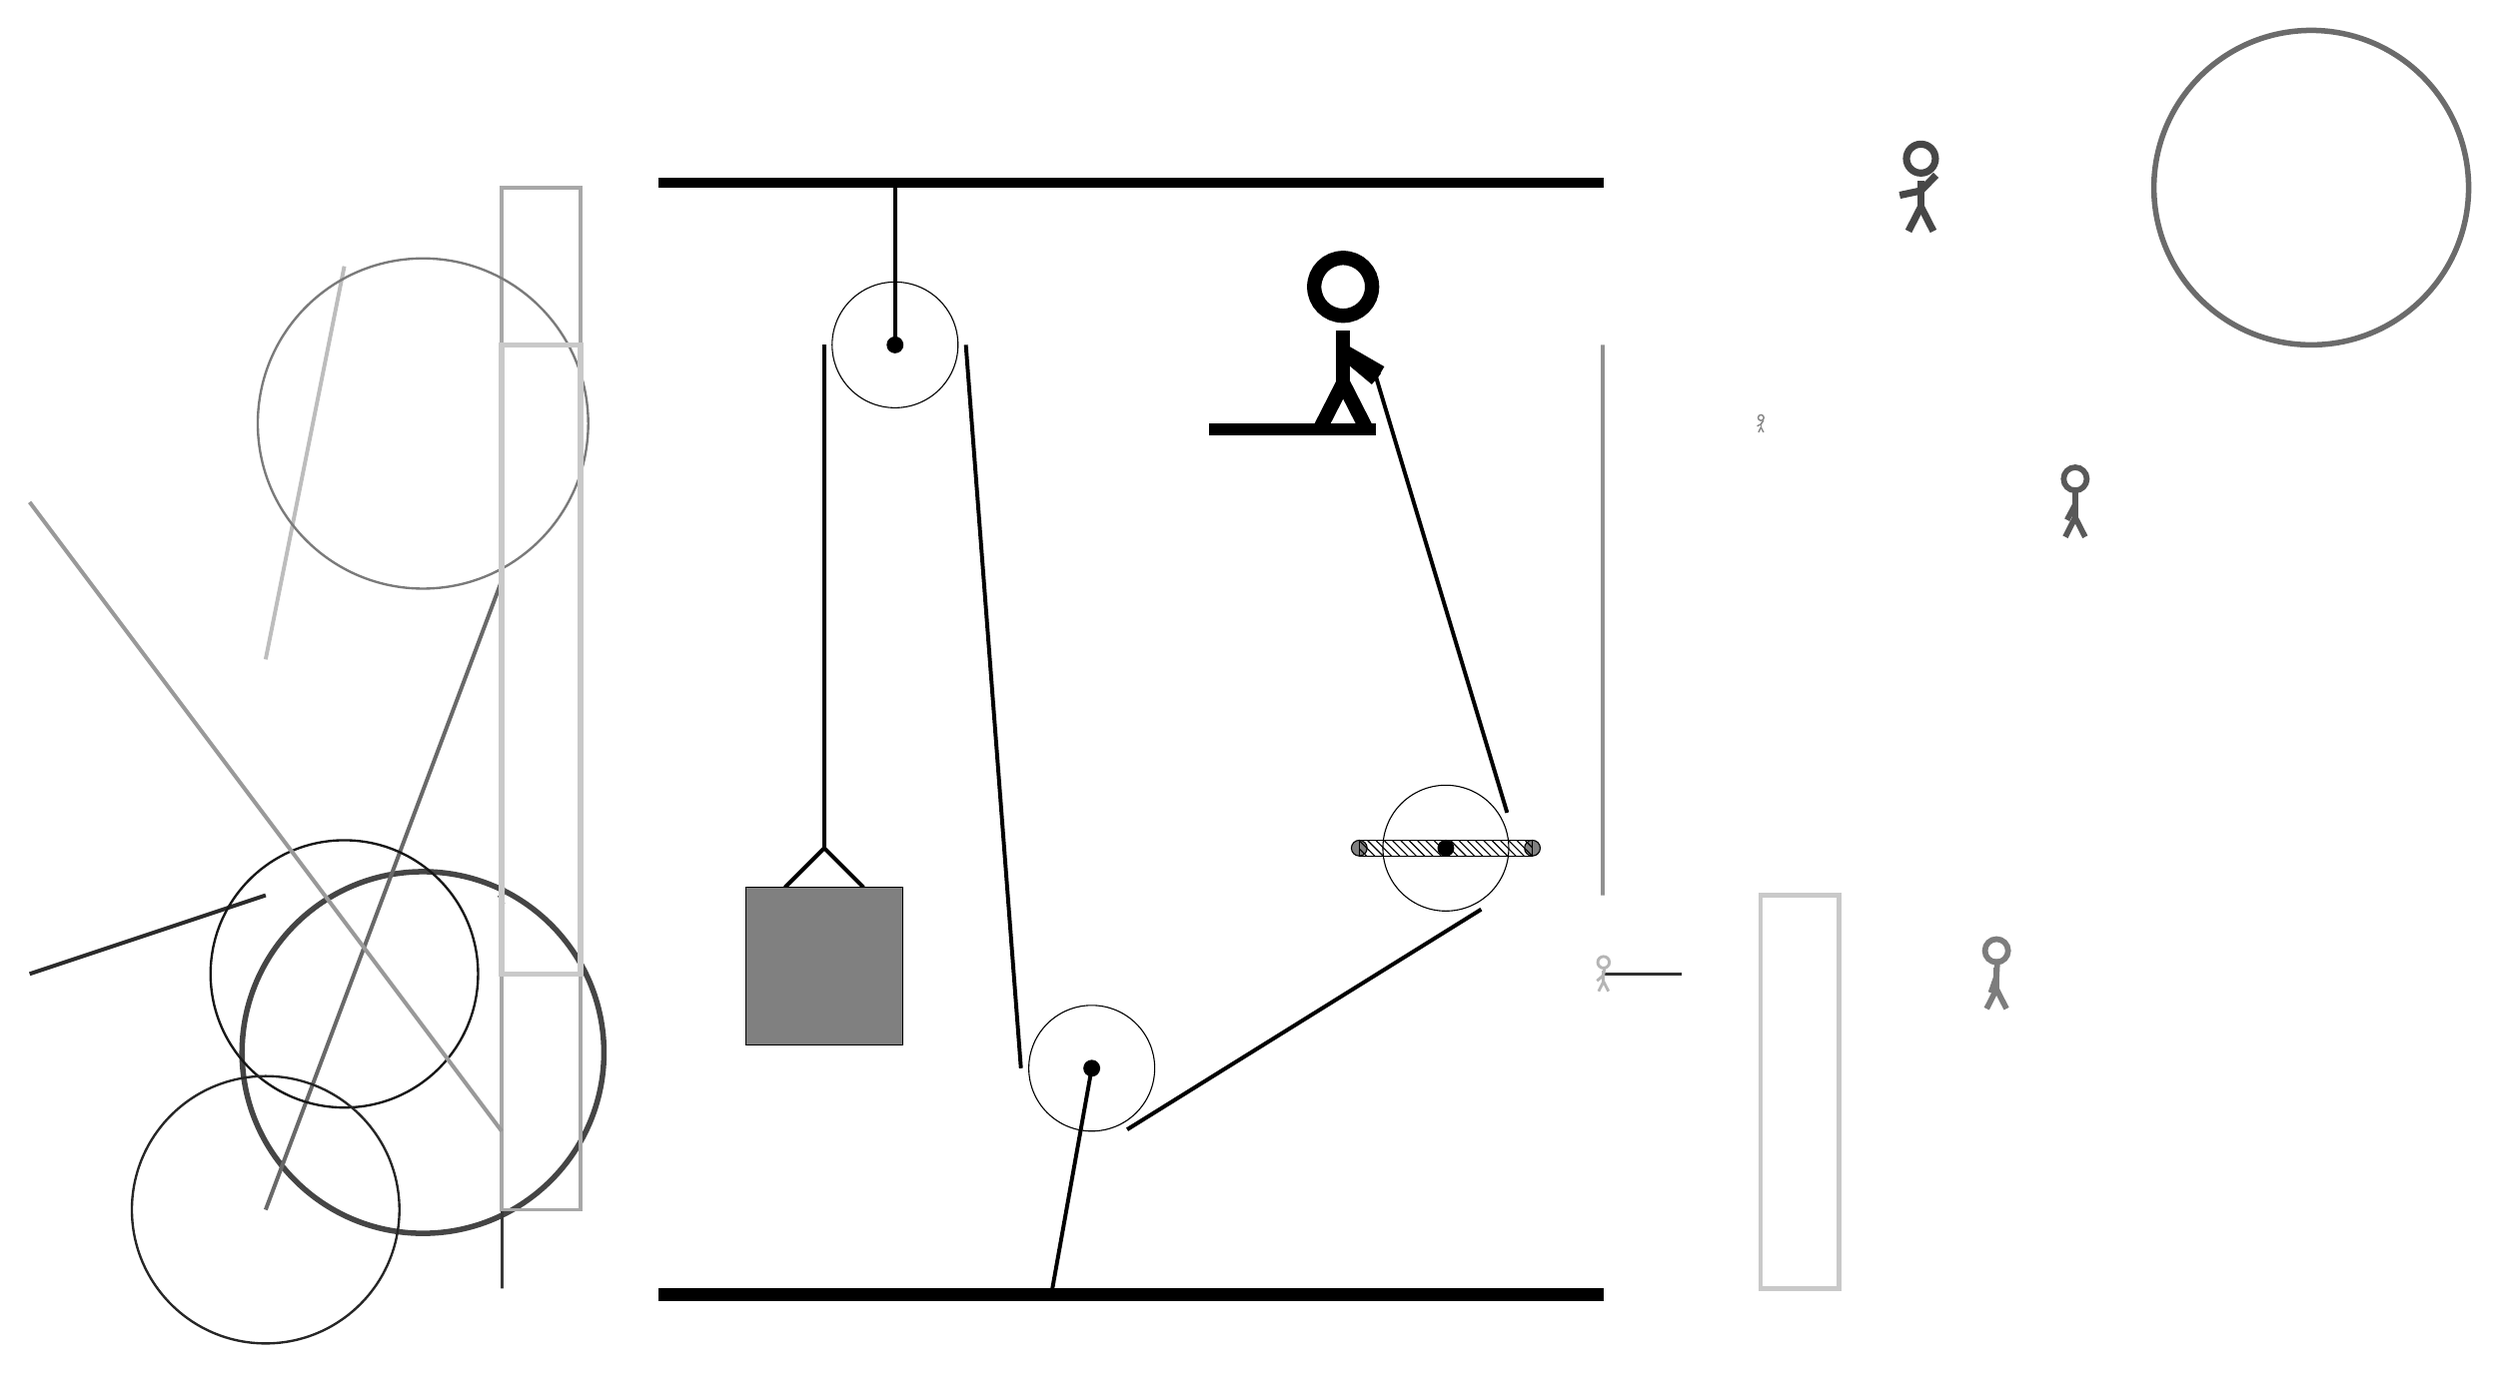
\begin{tikzpicture}
			%%%%% START %%%%%
			
			\draw[fill=black] (-2, 14) rectangle (10, 14.125);
			
			\draw (1, 12) circle (0.8);
			\draw[fill=black] (1, 12) circle (0.1);
			\draw[line width=0.5mm] (1, 14) -- (1, 12);
			
			\draw[line width=0.5mm, color=black!86](-3, 14) -- (-3, 14);
			
			\draw[line width=0.4mm, color=black!81] (11, 4) rectangle (10, 4);
			\draw[line width=0.5mm, color=black!43] (10, 12) rectangle (10, 5);
			\draw [line width=0.7mm, color=black!58](19, 14) circle (2.0);
			\draw [line width=0.7mm, color=black!73](-5, 3) circle (2.3);
			
			\draw[line width=0.5mm, color=black!59](-4, 9) -- (-7, 1);
			\draw [line width=0.2mm, color=black!99](-5, 4) circle (0.0);
			\draw[line width=0.4mm, color=black!78] (-4, 1) rectangle (-4, 0);
			\draw[line width=0.5mm, color=black!83](-7, 5) -- (-10, 4);
			\node[line width=0.5mm, color=black!65] at (16, 10) {\Strichmaxerl[4][62][89]};
			\draw[line width=0.5mm, color=black!26](-7, 8) -- (-6, 13);
			\node[line width=0.5mm, color=black!29] at (10, 4) {\Strichmaxerl[2][41][82]};
			\draw[line width=0.5mm, color=black!34] (-3, 1) rectangle (-4, 14);
			\node[line width=0.2mm, color=black!47] at (12, 11) {\Strichmaxerl[1][28][56]};
			\node[line width=0.2mm, color=black!72] at (14, 14) {\Strichmaxerl[5][12][46]};
			\draw [line width=0.3mm, color=black!52](-5, 11) circle (2.1);
			
			\node[line width=0.7mm, color=black!60] at (-4, 5) {\Strichmaxerl[1][9][31]};
			\draw [line width=0.3mm, color=black!91](-6, 4) circle (1.7);
			\draw[line width=0.6mm, color=black!21] (12, 5) rectangle (13, 0);
			\draw[line width=0.5mm, color=black!40](-4, 2) -- (-10, 10);
			\node[line width=0.4mm, color=black!51] at (15, 4) {\Strichmaxerl[4][71][87]};
			
			\draw[line width=0.7mm, color=black!21] (-4, 4) rectangle (-3, 12);
			\draw [line width=0.3mm, color=black!85](-7, 1) circle (1.7);
			
			\draw (3.5, 2.8) circle (0.8);
			\draw[fill=black] (3.5, 2.8) circle (0.1);
			\draw[line width=0.5mm] (3.5, 2.8) -- (3.0, 0);
			
			\draw[fill=white](8, 5.6) circle (0.8);
			\draw[fill=black] (8, 5.6) circle (0.1);
			\draw[fill=black!50] (9.1, 5.6) circle (0.1);
			\draw[fill=black!50] (6.9, 5.6) circle (0.1);
			\draw[pattern=north west lines, pattern color=black] (6.9, 5.7) rectangle (9.1, 5.5);
			
			\draw[line width=0.5mm](-0.4, 5.1) --  (0.1, 5.6) -- (0.6, 5.1);
			\draw[fill=black!50] (-0.9, 5.1) rectangle (1.1, 3.1);
			
			\draw[line width=0.5mm](0.1, 12) -- (0.1, 5.6);
			\centerarc[line width=0.5mm](1, 12)(180:0:0.9)
			\draw[line width=0.5mm](1.9, 12) -- (2.6, 2.8);
			\centerarc[line width=0.5mm](3.5, 2.8)(180:300:0.9);
			\draw[line width=0.5mm](3.95, 2.0206) -- (8.45, 4.8206);
			\centerarc[line width=0.5mm](8, 5.6)(300:390:0.9);
			\draw[line width=0.5mm](8.7794, 6.05) -- (7.05, 11.8);
			
			\node at (6.75, 12) {\Strichmaxerl[10][-220][-30]};
			\draw[fill=black] (5, 11) rectangle (7.1, 10.85);
			
			\draw[fill=black] (-2, 0) rectangle (10, -0.15);
			
			%%%%% END %%%%%
		\end{tikzpicture}
	\end{figure}	
\end{document}